\documentclass[11pt]{article}

% ---------------------------------------------------------------------------
% Telephony STT for AI Voice Agents -- self-contained LaTeX source.
% Compile: pdflatex -interaction=nonstopmode -halt-on-error paper.tex (run twice).
% Allowed packages only.
% ---------------------------------------------------------------------------
\usepackage[margin=1in]{geometry}
\usepackage{amsmath}
\usepackage{amssymb}
\usepackage{graphicx}
\usepackage{booktabs}
\usepackage{xcolor}
\usepackage{hyperref}
\usepackage{pgfplots}
\usepackage{tikz}
\pgfplotsset{compat=1.18}

\hypersetup{
  colorlinks=true,
  linkcolor=blue!50!black,
  citecolor=blue!50!black,
  urlcolor=blue!50!black,
  pdftitle={The Best Speech-to-Text Engine for AI Voice Agents on the Telephony Layer},
  pdfauthor={Mazin Salim, Mishahal Palakuniyil (MM Intelligence)}
}

% Engine palette (consistent across all per-engine figures).
\definecolor{cDeepgram}{HTML}{1F77B4}
\definecolor{cScribe}{HTML}{FF7F0E}
\definecolor{cSpeech}{HTML}{2CA02C}
\definecolor{cAAI}{HTML}{9467BD}
\definecolor{cCartesia}{HTML}{D62728}

\title{\textbf{The Best Speech-to-Text Engine for AI Voice Agents\\ on the Telephony Layer}\\[0.4em]
\large A Controlled Comparison of Five Streaming STT Engines\\ in One Identical PSTN Pipeline}

\author{%
  Mazin Salim \qquad Mishahal Palakuniyil\\[0.35em]
  \normalsize MM Intelligence\\
  \normalsize \texttt{mazin@mmintelligence.ai} \quad\textbullet\quad \texttt{mishal@mmintelligence.ai}%
}
\date{June 2026}

\begin{document}
\maketitle

% ===========================================================================
\begin{abstract}
\noindent
On the telephony layer, the latency of a speech-to-text (STT) engine is a
necessary but \emph{insufficient} property: the objective that actually matters
for an AI voice agent is \textbf{accuracy and reliability under real public
switched telephone network (PSTN) conditions}. We swapped five streaming STT
engines into one identical Pipecat telephony pipeline, holding turn-taking,
language model, text-to-speech, and the 8\,kHz audio path constant, and placed
roughly ten live Twilio phone calls per engine (about fifty total), each
requiring the assistant to capture a spoken name and a ten-digit callback
number. We find that speed does not predict accuracy: the fastest-median engine
(Cartesia Ink-Whisper) was the \emph{least} reliable, hallucinating nine
invented tokens and exhibiting a broken two-second latency tail. We also find
that one does not have to trade speed for accuracy. We recommend the stack
\textbf{Deepgram Nova-3 for STT paired with ElevenLabs Flash v2.5 for TTS} as
the primary choice for telephony voice agents. Deepgram's STT ties Speechmatics
for the best first-try number accuracy (70\%) with zero permanent number losses
and zero hallucination, yet runs at roughly half the latency of Speechmatics
(STT p50 0.374\,s vs.\ 0.777\,s), and it captured the hard name ``Mazin'' once
(fewer than AssemblyAI's three, but unlike Speechmatics' zero), so it delivers
accuracy, reliability, and speed in a single engine with no critical reliability
weakness, though AssemblyAI captures the hard name more often. We pair it with
ElevenLabs for synthesis because Deepgram's own Aura text-to-speech, not its
STT, interrupted and cut off speech on the telephony line; this also matches our
production deployment. \textbf{AssemblyAI Universal-3 Pro} is the runner-up and
leads proper-noun accuracy (three exact ``Mazin,'' the only engine to get the
brand acronym), while \textbf{Speechmatics Ursa (Enhanced)} is an
accuracy-focused alternative that ties on numbers (70\%) with the cleanest digit
formatting but runs $\sim$2$\times$ slower with no name-capture advantage.
\end{abstract}

% ===========================================================================
\section{Introduction}
\label{sec:intro}

Telephony is the hardest deployment surface for automatic speech recognition,
and an AI voice agent that answers phone calls lives or dies on that surface.
Four properties make it hard.

\textbf{Narrowband audio.} The PSTN delivers 8\,kHz mu-law audio. Half the
spectral information that wideband models are trained on is simply absent. No
amount of upsampling restores the missing high frequencies; it only changes the
container. An engine that is excellent on clean 16\,kHz microphone audio can
degrade sharply on a real phone call.

\textbf{Names and numbers are the hard tokens.} A receptionist's core job is to
capture \emph{entities}: a caller's name and a callback number. These are
exactly the tokens with the least linguistic redundancy. A language model can
repair a garbled common word from context; it cannot infer that ``\,016\,'' was
meant when the line delivered ``\,015\,''. Proper nouns are worse still, an
uncommon name like ``Mazin'' has essentially no language-model prior to lean
on, so the transcript is whatever the acoustic model emits.

\textbf{Latency is felt every turn.} In a spoken conversation, every turn pays
the STT's time-to-first-token (TTFB). Unlike batch transcription, where total
wall-clock time is amortized, conversational latency is experienced repeatedly
and directly as the gap before the agent responds. This makes TTFB a
first-class metric, but, as we show, not the \emph{only} one.

\textbf{Hallucination is a safety issue.} Some streaming models, when handed
unparseable narrowband audio, do not stay silent: they invent plausible tokens.
For a transcription product this is a quality nuisance. For a voice agent acting
on what it ``heard,'' a hallucinated phrase or a fabricated digit run is a
correctness and trust failure, the agent confidently stores or acts on
something the caller never said.

This paper argues a single thesis and supports it with controlled
measurements: \textbf{on the telephony layer, optimize for accuracy and
reliability, not raw speed; and you do not have to trade one for the other}.
Speed alone does not imply accuracy, the fastest engine here is the least
reliable, yet the best-balanced STT is also fast, so a slower engine buys no
accuracy advantage. Reliability also spans the whole stack, not the STT alone:
the agent must never hallucinate, must capture names and numbers correctly on a
noisy 8\,kHz line, and must not cut the caller off, a turn-taking property that,
as we found, lives in the text-to-speech layer as much as anywhere else.

% ===========================================================================
\section{Experimental Setup}
\label{sec:setup}

\subsection{The constant pipeline}
We built one Pipecat telephony pipeline and changed exactly one component, the
STT engine, across all conditions. Everything else was held fixed:

\begin{itemize}
  \item \textbf{Turn-taking:} Smart Turn V3 end-of-turn detection over Silero
        voice-activity detection (VAD), identical for every engine.
  \item \textbf{Language model:} Claude Haiku 4.5.
  \item \textbf{Text-to-speech:} ElevenLabs Flash v2.5.
  \item \textbf{Audio path:} Twilio PSTN at 8\,kHz mu-law, upsampled
        \emph{centrally} to a 16\,kHz container (\texttt{audio\_in\_sample\_rate
        = 16000}) before the STT, so every engine received bit-identical input
        framing. TTS output was rendered at 24\,kHz.
\end{itemize}

\subsection{Fairness controls}
Three controls protect the comparison. First, \textbf{no vocabulary or
keyterm seeding} was applied to any engine, no custom dictionaries, no boosted
phrases, no biasing toward the test name, number, or brand. This is the honest
out-of-the-box condition and it makes the hard-token results comparable.
Second, \textbf{central upsampling} guarantees identical audio framing rather
than letting each SDK resample differently. Third, \textbf{ground-truth
integrity}: each batch's STT processor class matched its label, so no engine's
output could be attributed to another (no cross-contamination of transcripts).

\subsection{Engines and configuration}
Table~\ref{tab:engines} lists the five engines and their exact streaming
configuration. All are run unseeded.

\begin{table}[ht]
\centering
\small
\begin{tabular}{@{}lll@{}}
\toprule
\textbf{Engine} & \textbf{Model / endpoint} & \textbf{Streaming configuration} \\
\midrule
Deepgram & Nova-3 (\texttt{nova-3-general}) & interim results; smart\_format; punctuate; \\
             & & endpointing 500\,ms \\
ElevenLabs & Scribe v2 Realtime & \texttt{scribe\_v2\_realtime}; manual commit \\
Speechmatics & Ursa, \textsc{Enhanced} & \texttt{turn\_detection\_mode=EXTERNAL}; \\
             & & include\_partials; max\_delay = server default \\
AssemblyAI & Universal-3 Pro Streaming & \texttt{u3-rt-pro}; \texttt{vad\_force\_turn\_endpoint=True} \\
Cartesia & Ink-Whisper (\texttt{ink-whisper}) & default streaming \\
\bottomrule
\end{tabular}
\caption{The five streaming STT engines and their configuration. Only this
component varied; all engines were run without vocabulary or keyterm seeding.}
\label{tab:engines}
\end{table}

\subsection{Instrumentation and the read-back accuracy proxy}
We instrument STT TTFB per turn and report its mean, median (p50), and 95th
percentile (p95). We also record the per-component medians for the LLM and TTS
so that STT latency can be placed in the context of the whole turn.

Because we deliberately ran \emph{without} ground-truth WER tooling, we measure
entity accuracy with an \textbf{AI read-back proxy}: the assistant repeats the
captured number back to the caller, and we score whether the spoken read-back
matches the true number. The speaker said the same ten-digit number,
\texttt{555-016-2049}, clearly on essentially every call, so a mismatch is
attributable to STT error rather than caller variation. The one exception is a
single AssemblyAI call in which the caller volunteered a \emph{different} number
than the standard one; because that call does not test the engine against the
fixed target, it is excluded from the integrity premise and flagged where it
affects scoring (Section~\ref{sec:numbers}). We score four outcomes per call:
correct on the \emph{first} try; \emph{fixed on retry} (the read-back-and-confirm
loop repaired it); \emph{never} correct (a permanently wrong stored number); and
\emph{eventual} success (correct by call end). Name and brand accuracy are
scored as exact-match captures of the target proper noun ``Mazin'' and the rare
phrase ``MM Intelligence.''

\subsection{Sample}
One single speaker placed roughly ten live Twilio (PSTN) calls per engine, about
fifty calls in total. The task on every call was identical: book an appointment
and provide a name and a ten-digit callback number. This sample is small and
single-speaker by design, enough to expose decisive reliability differences,
and we are explicit about its limits in Section~\ref{sec:limits}.

% ===========================================================================
\section{Results}
\label{sec:results}

\subsection{Latency}
\label{sec:lat}

Table~\ref{tab:latency} reports STT TTFB and the per-component medians.
The headline is that, \emph{end to end}, the engines are close: the top four by
total p50 fall within $\sim$108\,ms of one another (0.96--1.07\,s).
Speechmatics adds roughly 0.4--0.5\,s per turn at the STT stage. Cartesia is
\textbf{bimodal}: it has the fastest median (0.296\,s) but a p95 of 2.049\,s,
choking for about two seconds on disfluent input.

\begin{table}[ht]
\centering
\small
\begin{tabular}{@{}lrrrrrr@{}}
\toprule
\textbf{Engine} & \textbf{STT mean} & \textbf{STT p50} & \textbf{STT p95}
                & \textbf{LLM p50} & \textbf{TTS p50} & \textbf{TOTAL p50} \\
\midrule
Deepgram & 0.366 & 0.374 & 0.465 & 0.540 & 0.144 & 1.058 \\
Scribe & 0.340 & 0.345 & 0.393 & 0.587 & 0.139 & 1.071 \\
Speechmatics & 0.768 & 0.777 & 0.952 & 0.592 & 0.141 & 1.510 \\
AssemblyAI & 0.375 & 0.357 & 0.443 & 0.521 & 0.134 & 1.011 \\
Cartesia & 0.994 & \textbf{0.296} & \textbf{2.049} & 0.531 & 0.136 & 0.963 \\
\bottomrule
\end{tabular}
\caption{Latency in seconds. STT time-to-first-token (mean, p50, p95) plus
per-component medians. TOTAL p50 is the sum of medians (STT p50 + LLM p50 +
TTS p50), computed from the unrounded medians; it is an approximate composite,
\emph{not} a measured end-to-end percentile, and excludes turn-detection wait
and network time. (Because it uses unrounded inputs, the rounded AssemblyAI
parts may not visibly re-add to its printed total.) Bold marks Cartesia's
bimodal extremes: fastest median, broken tail.}
\label{tab:latency}
\end{table}

Figure~\ref{fig:ttfb} shows the TTFB p50/p95 bars. Cartesia's p95 tail and
Speechmatics' higher-but-stable bars are both visible; the other three sit
tightly under 0.47\,s at p95. Figure~\ref{fig:stack} stacks the per-turn
medians and makes the structural point: STT is a \emph{minority} of the turn
budget, and the engines are nearly indistinguishable end to end, so optimizing
STT purely for speed buys little while risking the reliability axis.

% --- Figure 1: grouped ybar TTFB p50/p95 ---
% Statistic series use palette-neutral grays so engine brand colors stay
% reserved for the per-engine charts (scatter, stacks, reliability).
\begin{figure}[ht]
\centering
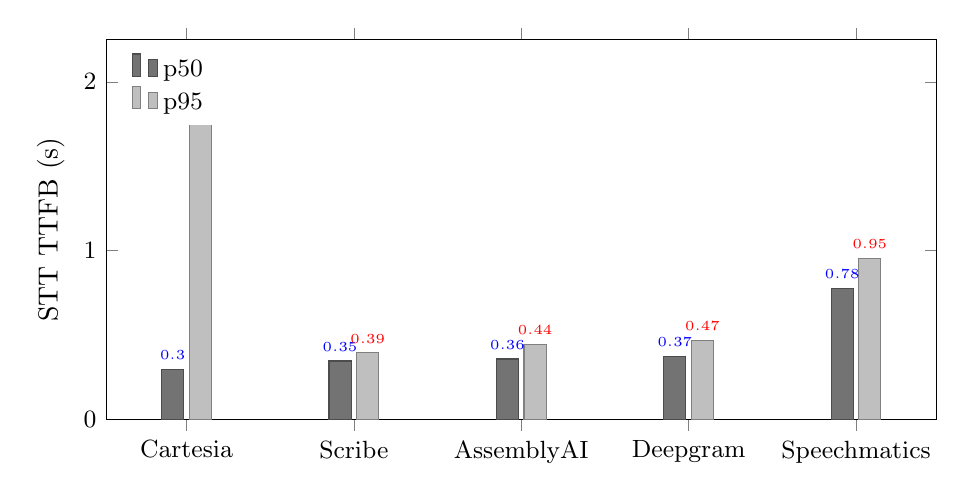
\begin{tikzpicture}
\begin{axis}[
    width=\linewidth, height=6.4cm,
    ybar, bar width=8pt,
    enlarge x limits=0.12,
    symbolic x coords={Cartesia,Scribe,AssemblyAI,Deepgram,Speechmatics},
    xtick=data,
    ymin=0, ymax=2.25,
    ylabel={STT TTFB (s)},
    nodes near coords, nodes near coords align={vertical},
    every node near coord/.append style={font=\tiny, /pgf/number format/fixed,
        /pgf/number format/precision=2},
    legend style={at={(0.02,0.98)}, anchor=north west, font=\small, draw=none},
    legend cell align=left,
    tick label style={font=\small},
]
\addplot+[fill=black!55, draw=black!70] coordinates
    {(Cartesia,0.296) (Scribe,0.345) (AssemblyAI,0.357) (Deepgram,0.374) (Speechmatics,0.777)};
\addplot+[fill=black!25, draw=black!50] coordinates
    {(Cartesia,2.049) (Scribe,0.393) (AssemblyAI,0.443) (Deepgram,0.465) (Speechmatics,0.952)};
\legend{p50, p95}
\end{axis}
\end{tikzpicture}
\caption{STT time-to-first-token, p50 vs.\ p95, per engine (ascending by p50).
The two statistic series use neutral grays so that engine brand colors remain
reserved for the per-engine charts; near-coordinate labels are shown to two
decimals, with the exact three-decimal figures in Table~\ref{tab:latency}.
Cartesia owns the fastest median yet a 2.049\,s p95 tail, a broken worst case.
Speechmatics' bars are the tallest but tight (p50 0.777\,s, p95 0.952\,s):
slower, but stable and predictable.}
\label{fig:ttfb}
\end{figure}

% --- Figure 2: stacked bar total latency ---
\begin{figure}[ht]
\centering
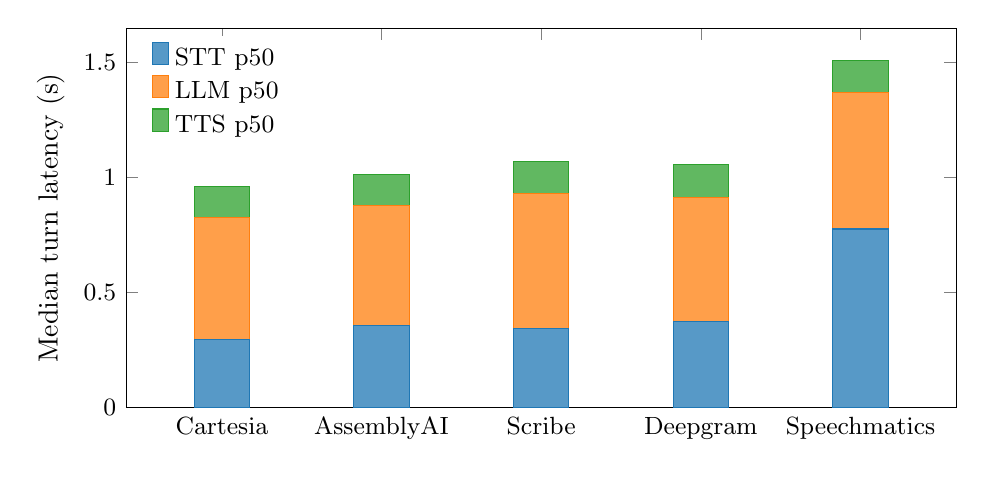
\begin{tikzpicture}
\begin{axis}[
    width=\linewidth, height=6.4cm,
    ybar stacked, bar width=20pt,
    enlarge x limits=0.15,
    symbolic x coords={Cartesia,AssemblyAI,Scribe,Deepgram,Speechmatics},
    xtick=data,
    ymin=0, ymax=1.65,
    ylabel={Median turn latency (s)},
    legend style={at={(0.02,0.98)}, anchor=north west, font=\small, draw=none},
    legend cell align=left,
    tick label style={font=\small},
]
\addplot+[fill=cDeepgram!75, draw=cDeepgram] coordinates
    {(Cartesia,0.296) (AssemblyAI,0.357) (Scribe,0.345) (Deepgram,0.374) (Speechmatics,0.777)};
\addplot+[fill=cScribe!75, draw=cScribe] coordinates
    {(Cartesia,0.531) (AssemblyAI,0.521) (Scribe,0.587) (Deepgram,0.540) (Speechmatics,0.592)};
\addplot+[fill=cSpeech!75, draw=cSpeech] coordinates
    {(Cartesia,0.136) (AssemblyAI,0.134) (Scribe,0.139) (Deepgram,0.144) (Speechmatics,0.141)};
\legend{STT p50, LLM p50, TTS p50}
\end{axis}
\end{tikzpicture}
\caption{Per-turn latency budget, stacked medians (STT + LLM + TTS). STT is a
minority of every turn. The four non-Speechmatics engines land within
$\sim$108\,ms end to end (0.96--1.07\,s); Speechmatics' extra cost is confined
to the STT segment. Composite of medians, not a measured end-to-end percentile.}
\label{fig:stack}
\end{figure}

\subsection{Number accuracy}
\label{sec:numbers}

Table~\ref{tab:numbers} reports read-back accuracy for the callback number.
Speechmatics and Deepgram tie for the best first-try number accuracy (70\%),
both with zero permanent losses; Speechmatics retains a distinct edge in the
cleanest auto-formatting (\texttt{(555)\,016-2049}). The first-try gap among the
top three (70/70/50\%) spans only about one call and is within noise; we do not
over-rank it.

The decisive column is \textbf{never}, a permanently wrong stored number, the
failure a receptionist cannot walk back. Only AssemblyAI (1) and Cartesia (1)
ever lost a number permanently; Speechmatics, Deepgram, and Scribe lost none.
The assistant's read-back-and-confirm loop is what lifts every engine to
90--100\% eventual accuracy, which is precisely why a single first-try number
does not settle the ranking but a single permanent loss does.

Two of these counts rest on call-level judgment and we make them explicit.
AssemblyAI's lone permanent ``loss'' is a borderline case: on that call the
caller actually volunteered a \emph{different} number than the standard
\texttt{555-016-2049} and the agent captured and confirmed it correctly, so it
is not strictly an STT failure against the fixed target. We retain it in the
``never'' count conservatively (the agent did not end the call holding the
standard number) but flag that excluding it would make AssemblyAI 4/9 first-try,
never\,=\,0, eventual 100\%.\footnote{This is the single call that motivates the
softened integrity premise in Section~\ref{sec:setup}: the standard number was
\emph{not} spoken on it, so it does not test the engine against the constant
target.} Cartesia's permanent loss is the call in which a wrong number was
affirmatively confirmed mid-conversation before a later correct read-back; a
naive ``final read-back'' check would miss it and score Cartesia
never\,=\,0.\footnote{The Cartesia read-back transcript for this call is
non-monotonic in time: a wrong number (\,``\,\dots five five nine, zero one, one
four one\,'') is confirmed before a later correct read-back of
\texttt{5550162049} appears. The permanent loss is counted because a wrong
number was affirmatively confirmed, not because the call ends incorrectly.}

\begin{table}[ht]
\centering
\small
\begin{tabular}{@{}lrrrrr@{}}
\toprule
\textbf{Engine} & \textbf{First-try} & \textbf{Fixed on retry} & \textbf{Never}
                & \textbf{Eventual} & \textbf{Note} \\
\midrule
Speechmatics & 7/10 (70\%) & 3 & \textbf{0} & 100\% & cleanest formatting \\
Deepgram & 7/10 (70\%) & 3 & \textbf{0} & 100\% & ties best first-try \\
Scribe & 5/10 (50\%) & 5 & \textbf{0} & 100\% & \\
AssemblyAI & 4/10 (40\%) & 5 & \textbf{1} & 90\% & loss is a different-number call \\
Cartesia & 2/10 (20\%) & 7 & \textbf{1} & 90\% & loss confirmed mid-call \\
\bottomrule
\end{tabular}
\caption{Callback-number read-back accuracy (standard number
\texttt{555-016-2049}, spoken identically on every call except one AssemblyAI
call where the caller gave a different number). ``Never'' counts permanently
wrong stored numbers and is the decisive reliability column. Speechmatics and
Deepgram tie for the best first-try accuracy (70\%); see the footnotes in
Section~\ref{sec:numbers} for the two judgment-dependent ``never'' counts.}
\label{tab:numbers}
\end{table}

Figure~\ref{fig:scatter} is the thesis figure. It plots STT p50 latency against
first-try number accuracy. There is \textbf{no positive correlation between
speed and accuracy}: Cartesia is the fastest yet least accurate (0.296\,s,
20\%); Speechmatics is the slowest yet most accurate (0.777\,s, 70\%). We draw
no trend line because there is no trend to draw. Figure~\ref{fig:numbars}
contrasts first-try and eventual number accuracy and shows how the confirm loop
compresses the field at the eventual stage, while leaving the two engines with
permanent losses capped at 90\%.

% --- Figure 3: scatter, the thesis figure ---
\begin{figure}[ht]
\centering
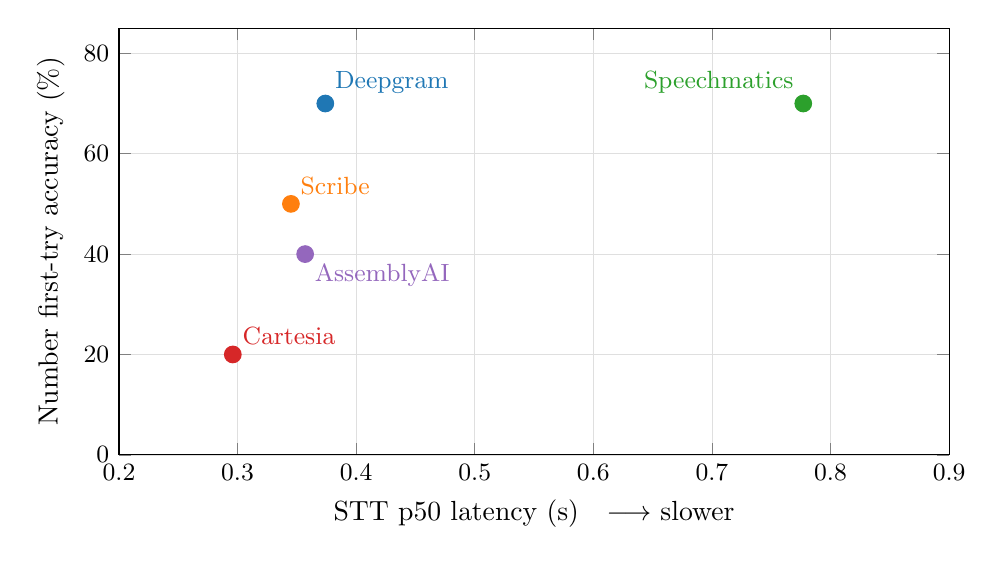
\begin{tikzpicture}
\begin{axis}[
    width=\linewidth, height=7.0cm,
    xlabel={STT p50 latency (s)\quad$\longrightarrow$ slower},
    ylabel={Number first-try accuracy (\%)},
    xmin=0.2, xmax=0.9,
    ymin=0, ymax=85,
    grid=both, grid style={line width=0.2pt, draw=gray!25},
    tick label style={font=\small},
    every node near coord/.append style={font=\small},
    scatter/classes={a={mark=*,draw=black}},
]
% one point per engine, colored + labeled
\addplot[only marks, mark=*, mark size=3pt, color=cCartesia]
    coordinates {(0.296,20)};
\node[anchor=south west, font=\small, color=cCartesia] at (axis cs:0.296,20) {Cartesia};
\addplot[only marks, mark=*, mark size=3pt, color=cScribe]
    coordinates {(0.345,50)};
\node[anchor=south west, font=\small, color=cScribe] at (axis cs:0.345,50) {Scribe};
\addplot[only marks, mark=*, mark size=3pt, color=cAAI]
    coordinates {(0.357,40)};
\node[anchor=north west, font=\small, color=cAAI] at (axis cs:0.357,40) {AssemblyAI};
\addplot[only marks, mark=*, mark size=3pt, color=cDeepgram]
    coordinates {(0.374,70)};
\node[anchor=south west, font=\small, color=cDeepgram] at (axis cs:0.374,70) {Deepgram};
\addplot[only marks, mark=*, mark size=3pt, color=cSpeech]
    coordinates {(0.777,70)};
\node[anchor=south east, font=\small, color=cSpeech] at (axis cs:0.777,70) {Speechmatics};
\end{axis}
\end{tikzpicture}
\caption{The thesis figure: STT p50 latency vs.\ first-try number accuracy. One
labeled point per engine. Fastest $\neq$ most accurate, Cartesia is fastest yet
least accurate (bottom-left), while Speechmatics and Deepgram tie for the best
first-try accuracy (70\%) at opposite ends of the latency axis (Speechmatics
slowest, top-right; Deepgram far faster at the same height). There is no
positive speed--accuracy correlation, so no trend line is drawn.}
\label{fig:scatter}
\end{figure}

% --- Figure 4: grouped bar first-try vs eventual number accuracy ---
\begin{figure}[ht]
\centering
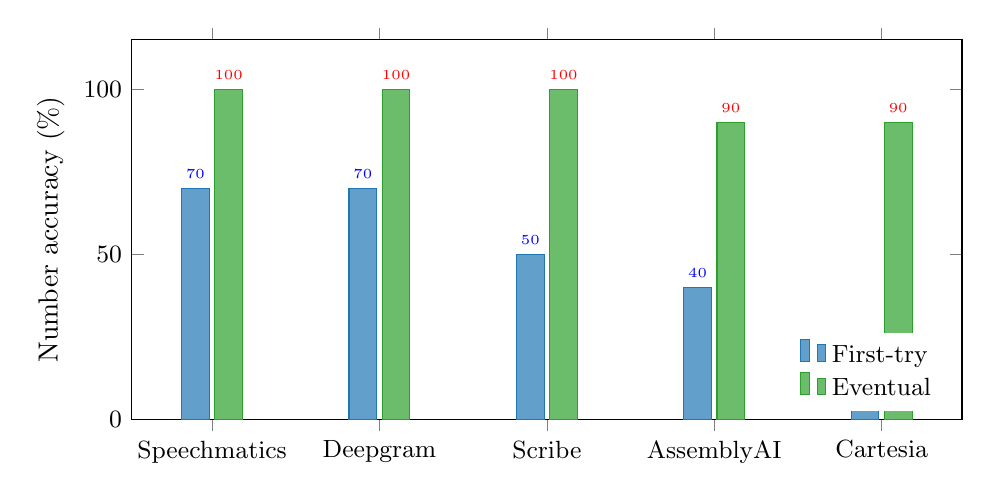
\begin{tikzpicture}
\begin{axis}[
    width=\linewidth, height=6.4cm,
    ybar, bar width=10pt,
    enlarge x limits=0.12,
    symbolic x coords={Speechmatics,Deepgram,Scribe,AssemblyAI,Cartesia},
    xtick=data,
    ymin=0, ymax=115,
    ylabel={Number accuracy (\%)},
    nodes near coords, nodes near coords align={vertical},
    every node near coord/.append style={font=\tiny},
    legend style={at={(0.98,0.02)}, anchor=south east, font=\small, draw=none},
    legend cell align=left,
    tick label style={font=\small},
]
\addplot+[fill=cDeepgram!70, draw=cDeepgram] coordinates
    {(Speechmatics,70) (Deepgram,70) (Scribe,50) (AssemblyAI,40) (Cartesia,20)};
\addplot+[fill=cSpeech!70, draw=cSpeech] coordinates
    {(Speechmatics,100) (Deepgram,100) (Scribe,100) (AssemblyAI,90) (Cartesia,90)};
\legend{First-try, Eventual}
\end{axis}
\end{tikzpicture}
\caption{Number accuracy: first-try vs.\ eventual, per engine. The
read-back-and-confirm loop lifts every engine to 90--100\% eventual, but
AssemblyAI and Cartesia are capped at 90\% by their single permanent losses,
while the three loss-free engines reach 100\%.}
\label{fig:numbars}
\end{figure}

\subsection{Name accuracy}
\label{sec:names}

Proper nouns separate the engines where digits compress them.
Table~\ref{tab:names} reports exact captures of the target name ``Mazin'' and
lists the raw \texttt{caller\_names} each engine produced. AssemblyAI is the
clear leader with three exact ``Mazin'' captures; Scribe, Cartesia, and Deepgram
manage one each; only Speechmatics never captured it exactly, returning
near-misses such as ``Maison'' and ``Mohsen.'' Common names
(Emma, Tommy, Michelle) were handled well by all engines and are
non-discriminating at this sample size.

\begin{table}[ht]
\centering
\small
\begin{tabular}{@{}lcl@{}}
\toprule
\textbf{Engine} & \textbf{Exact ``Mazin''} & \textbf{Captured \texttt{caller\_names} (raw)} \\
\midrule
AssemblyAI & \textbf{3} & Mazin\,$\times$3, Emma, Tommy, Michelle, Nabi \\
Scribe & 1 & Mazin, Martin, Neha, Navy, Jack, Tommy, Josh, Michelle, \\
             & & Emma, Nicolas Cage \\
Cartesia & 1 & Mazin, Mazza, Mazen, Mazen Saleem, Basen, Emma, John, Tom \\
Deepgram & 1 & Mazin, Maazel, Mazan Salim, Maazen, Austin, Tommy, \\
             & & Michelle, Neha, Salim, Bright \\
Speechmatics & 0 & Maison, Maison, James, Emma, Mohsen, Mohsen, Jack, \\
             & & Vanessa, Hannah \\
\bottomrule
\end{tabular}
\caption{Exact captures of the hard proper noun ``Mazin'' (the speaker's real
name) and the raw captured names per engine, unseeded. AssemblyAI leads
entity capture; Deepgram lands the hard name once, while Speechmatics misses it
entirely.}
\label{tab:names}
\end{table}

\subsection{Brand / rare phrase}
\label{sec:brand}

Table~\ref{tab:brand} reports how each engine rendered the rare phrase ``MM
Intelligence'', specifically the word before ``intelligence.'' Only AssemblyAI
ever produced the correct ``mm'' acronym (and only once, among three ``mm''
renderings). Every other engine substituted plausible but wrong tokens
(``ml,'' ``of,'' ``amazon,'' ``artificial,'' ``animal''). Unseeded, a novel
brand acronym is near-impossible for narrowband STT, further evidence that
entity capture, not raw speed, is the binding constraint.

\begin{table}[ht]
\centering
\small
\begin{tabular}{@{}ll@{}}
\toprule
\textbf{Engine} & \textbf{Rendering of the word before ``intelligence''} \\
\midrule
AssemblyAI & mm\,$\times$3 (only one correct) \\
Cartesia & mm\,$\times$1 \\
Deepgram & of\,/\,mim \\
Scribe & mm\,/\,artificial\,/\,amazon\,/\,animal\,$\times$2\,/\,m \\
Speechmatics & ml\,$\times$2\,/\,mlm\,/\,with\,$\times$3\,/\,m \\
\bottomrule
\end{tabular}
\caption{Rendering of the rare brand phrase ``MM Intelligence'' (target word:
``MM''). Only AssemblyAI produced a correct ``mm''; all engines otherwise
substituted. ``mm'' captures are counted leniently, they include
hyphenated/split forms such as ``M-M'' and ``Emma M.'', and ``only one
correct'' for AssemblyAI is a manual case/spacing judgment not derivable from
the lowercased transcript text alone. Unseeded, novel acronyms are a known hard
case.}
\label{tab:brand}
\end{table}

\subsection{Hallucination}
\label{sec:halluc}

Table~\ref{tab:halluc} is the sharpest reliability separator. We counted
invented ``whatever'' tokens, content the model emitted for unparseable
narrowband audio that the caller never said. \textbf{Cartesia produced nine};
every other engine produced \emph{zero}. Cartesia additionally emitted
repeated-digit runs (e.g.\ ``016-016-016,'' ``0-1-6-9-9-9-9''), the Whisper
failure mode of filling silence or noise with fabricated structure. For a voice
agent this is disqualifying: the agent acts on tokens that were never spoken.

\begin{table}[ht]
\centering
\small
\begin{tabular}{@{}lcl@{}}
\toprule
\textbf{Engine} & \textbf{Invented tokens} & \textbf{Other artifacts} \\
\midrule
Cartesia & \textbf{9} & repeated-digit runs (016-016-016; 0-1-6-9-9-9-9) \\
Deepgram & 0 &, \\
Scribe & 0 &, \\
Speechmatics & 0 &, \\
AssemblyAI & 0 &, \\
\bottomrule
\end{tabular}
\caption{Hallucinated (``whatever'') tokens invented in caller turns. Cartesia
fabricated nine and emitted repeated-digit runs; all other engines hallucinated
nothing.}
\label{tab:halluc}
\end{table}

\subsection{Reliability summary}
\label{sec:relsum}

Table~\ref{tab:reliability} consolidates the failure modes that actually break a
receptionist, and Figure~\ref{fig:reliability} visualizes the three decisive
axes together. Cartesia's hallucination spike and broken latency tail, and
AssemblyAI's name-capture lead, are both immediately visible. Deepgram is clean
on every measured STT reliability axis (zero permanent losses, zero
hallucination, one hard-name capture) while also posting a sub-second, stable
tail, the only engine to combine top-tier accuracy with low latency.

\begin{table}[ht]
\centering
\small
\begin{tabular}{@{}lccccc@{}}
\toprule
\textbf{Failure mode} & \textbf{Speechmatics} & \textbf{AssemblyAI}
                      & \textbf{Deepgram} & \textbf{Scribe} & \textbf{Cartesia} \\
\midrule
Permanent number loss & \textbf{0} & 1 & \textbf{0} & \textbf{0} & 1 \\
Hallucination (tokens) & \textbf{0} & \textbf{0} & \textbf{0} & \textbf{0} & 9 \\
Latency tail p95 (s) & 0.952 & 0.443 & \textbf{0.465} & 0.393 & 2.049 \\
Exact name captures & 0 & \textbf{3} & 1 & 1 & 1 \\
\bottomrule
\end{tabular}
\caption{Reliability summary across the failure modes that break a phone
receptionist (all STT failure modes). The two permanent number losses are the
judgment-dependent calls footnoted in Section~\ref{sec:numbers}. Bold in the
latency-tail row marks Deepgram's recommended best-balanced profile, not the row
minimum (Scribe's 0.393\,s p95 is the lowest in that row). Deepgram has zero
permanent losses, zero hallucination, a hard-name capture (though AssemblyAI
leads name capture 3 to 1), and a sub-second, stable tail, the best balance of
accuracy and speed; Speechmatics matches it on the two failure axes but at
$\sim$2$\times$ the latency. The caller-cut-off behavior we observed was a
property of the text-to-speech layer, not the STT (Section~\ref{sec:disc}), so
it is not an STT failure mode here.}
\label{tab:reliability}
\end{table}

% --- Figure 5: grouped bar reliability failure modes ---
\begin{figure}[ht]
\centering
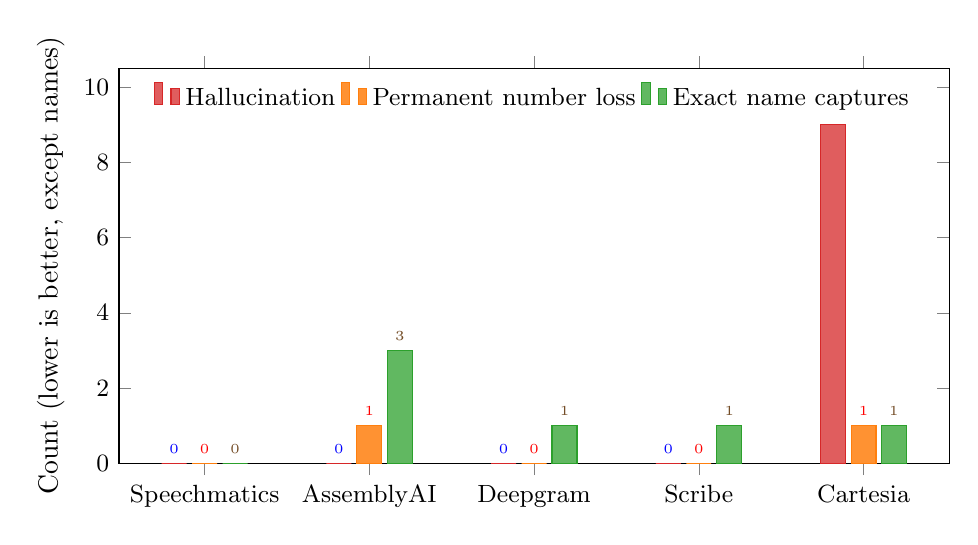
\begin{tikzpicture}
\begin{axis}[
    width=\linewidth, height=6.6cm,
    ybar, bar width=9pt,
    enlarge x limits=0.13,
    symbolic x coords={Speechmatics,AssemblyAI,Deepgram,Scribe,Cartesia},
    xtick=data,
    ymin=0, ymax=10.5,
    ylabel={Count (lower is better, except names)},
    nodes near coords, nodes near coords align={vertical},
    every node near coord/.append style={font=\tiny},
    legend style={at={(0.5,0.98)}, anchor=north, legend columns=3, font=\small, draw=none},
    legend cell align=left,
    tick label style={font=\small},
]
\addplot+[fill=cCartesia!75, draw=cCartesia] coordinates
    {(Speechmatics,0) (AssemblyAI,0) (Deepgram,0) (Scribe,0) (Cartesia,9)};
\addplot+[fill=cScribe!85, draw=cScribe] coordinates
    {(Speechmatics,0) (AssemblyAI,1) (Deepgram,0) (Scribe,0) (Cartesia,1)};
\addplot+[fill=cSpeech!75, draw=cSpeech] coordinates
    {(Speechmatics,0) (AssemblyAI,3) (Deepgram,1) (Scribe,1) (Cartesia,1)};
\legend{Hallucination, Permanent number loss, Exact name captures}
\end{axis}
\end{tikzpicture}
\caption{Reliability failure modes per engine. Hallucination and permanent
number loss are failures (lower is better); exact name captures are a benefit
(higher is better). Cartesia's hallucination spike (9) dominates the chart;
AssemblyAI leads exact name captures (3); Speechmatics shows no failures on
either failure axis.}
\label{fig:reliability}
\end{figure}

\subsection{Ground-truth integrity}
\label{sec:gt}

Two facts protect the integrity of these numbers. The callback number was the
\emph{same} on essentially every call, the one documented exception is the
single AssemblyAI call in which the caller volunteered a different number
(Section~\ref{sec:numbers}), so number misses are STT errors, not caller
variation. And each batch's STT processor class matched its label, so no
transcript from one engine was attributed to another. We do not claim a
ground-truth word error rate; the entity metrics above are exact-match scores
against known targets, which is the relevant unit for a receptionist anyway, a
name or number is either right or it is not.

% ===========================================================================
\section{Discussion}
\label{sec:disc}

\paragraph{Optimize for accuracy and reliability, and you need not trade away
speed.}
The latency results (Section~\ref{sec:lat}) and the thesis figure
(Figure~\ref{fig:scatter}) make the central claim concrete. Speed does not imply
accuracy: the fastest-median engine, Cartesia, was the least reliable on every
accuracy and safety axis we measured. But the inverse trap is just as real, and
the data refutes it. You do \emph{not} have to buy accuracy with latency.
Deepgram delivers accuracy, reliability, \emph{and} speed in one engine: it ties
Speechmatics for the best first-try numbers (70\%) with zero permanent losses
and zero hallucination, lands the hard name once, and does it at roughly half
Speechmatics' STT latency (p50 0.374\,s vs.\ 0.777\,s). Speechmatics' extra
$\sim$2$\times$ at the STT stage therefore buys no accuracy advantage over
Deepgram. Because STT is a minority of the turn budget
(Figure~\ref{fig:stack}) and the field is within $\sim$108\,ms end to end,
shaving STT milliseconds at the cost of reliability is a bad trade, but so is
paying latency for accuracy you can already get faster. Latency is a floor
requirement, not the optimization target, and here the most accurate STT is also
one of the fastest.

\paragraph{For a voice agent, performance \emph{is} reliability, across the whole
stack.}
The properties that decide whether a phone agent is usable are not captured by a
single accuracy headline. They are: never hallucinating, capturing names and
numbers correctly on a noisy 8\,kHz line, and never cutting the caller off.
Reframed this way, ``the best STT'' is the one that fails the least in the ways
that break a receptionist, which is exactly how Table~\ref{tab:reliability}
ranks them. But reliability is a property of the \emph{stack}, not the STT in
isolation: as we discuss below, the caller-cut-off behavior we observed came
from the text-to-speech engine, not the recognizer, so the reliable
configuration is a reliable STT paired with a reliable TTS.

\paragraph{The best-balanced STT: Deepgram Nova-3.}
Deepgram's STT is the best-balanced engine in the study: no critical reliability
weakness, and competitive on both entity axes. Its numbers are top-tier: 70\%
first-try number accuracy, which \emph{ties Speechmatics for the best in the
field}, zero permanent losses, and zero hallucination. It also lands the hard
name ``Mazin'' once, where Speechmatics never did, so it avoids the zero on both
entity axes, solid on numbers and at least non-zero on the hard name, though
AssemblyAI captures that name more often (three vs.\ one). And it does all of
this fast: STT p50 0.374\,s, roughly half Speechmatics' 0.777\,s, with a tight
0.465\,s p95. It is the only engine that combines best-in-class number accuracy,
zero hallucination, a hard-name capture, and low, stable latency at once. That
is why we make Deepgram STT the primary recommendation, and pair it with
ElevenLabs for synthesis (next paragraph), which is also the configuration we run
in production.

\paragraph{Reliability spans the stack: the cut-off behavior was the TTS, not the
STT.}
Reliability on telephony has an axis that isolated STT transcription metrics do
not see: whether the agent cuts the caller off. In our telephony testing we
observed exactly that failure, the agent interrupting and clipping speech, but
on tracing it the cause was the \emph{text-to-speech} layer, not the recognizer.
Deepgram's own Aura TTS exhibited interruption and speech-cut-off behavior on the
line, which, together with lower output quality, is why we synthesize with
ElevenLabs Flash v2.5 rather than Aura. We present this as a \emph{qualitative,
observed} field finding that motivated the TTS choice. The present benchmark
held TTS constant at ElevenLabs across all five STT conditions and therefore did
\emph{not} measure Aura's interruptions; we did not instrument a numeric
interruption rate for Aura, and we do not invent one. Quantifying TTS barge-in
behavior under controlled conditions is future work. The lesson is that strong
STT metrics in isolation do not equal a reliable telephony agent: reliability is
a property of the whole stack, and the reliable stack here is Deepgram STT paired
with ElevenLabs TTS.

\paragraph{The names-vs-numbers trade-off, and why Deepgram resolves it.}
The cleanest mirror image runs between two engines. AssemblyAI led proper nouns
(three exact ``Mazin,'' the only correct brand acronym) but trailed on first-try
numbers (40\%) and took one permanent number loss. Speechmatics inverted that
profile exactly: best (tied) numbers and cleanest digit formatting, zero
permanent losses, but the only engine with zero exact captures of the hard name.
Deepgram sits between the two poles and, crucially, does not pay for it in
latency: it ties Speechmatics for the best first-try numbers (70\%, zero
permanent losses) \emph{and} lands the hard name once, so it avoids the zero on
both entity axes at once while running at roughly half Speechmatics' STT latency.
That is why Deepgram is the best-balanced default rather than a niche pick. The
two remaining engines are specialists. Speechmatics is the
\textbf{accuracy-focused alternative}: it matches Deepgram on numbers and has the
cleanest digit auto-formatting, but it is $\sim$2$\times$ slower and never
captured ``Mazin'' exactly, so its added latency buys no accuracy advantage over
Deepgram, recommend it only where digit formatting matters most and latency is
irrelevant. AssemblyAI is the \textbf{best pick for names}: choose it when
proper-noun fidelity dominates and the weaker first-try number accuracy (40\%,
one permanent loss) is acceptable.

\paragraph{Fixable vs.\ unfixable errors, and the case for seeding.}
A first-try number miss is \emph{fixable}: the read-back-and-confirm loop
repaired enough of them to lift every engine to 90--100\% eventual accuracy
(Figure~\ref{fig:numbars}). A permanent loss and a hallucination are
\emph{unfixable} at the conversation layer, the agent stores or acts on wrong
content without ever knowing. This distinction is why we weight the ``never''
and hallucination columns far above first-try differences of one call. It also
points at the most obvious next lever: we ran every engine \emph{unseeded}, and
the worst residual errors were hard proper nouns and a novel brand acronym,
exactly the tokens that vocabulary/keyterm seeding targets. Seeding the name,
the brand, and digit-formatting hints should compress the name and brand gaps
materially and is the first thing to add before any production deployment.

\paragraph{Cartesia is concrete proof that speed $\neq$ reliability.}
Cartesia had the fastest median TTFB and was nonetheless disqualifying on
telephony: nine hallucinated tokens, fabricated repeated-digit runs, a
permanent number loss, the worst first-try number accuracy (20\%), and a broken
2.049\,s p95 tail. It is the cleanest single counterexample to the assumption
that the fastest STT is the best STT.

\paragraph{TTS note (design choice, not an STT result).}
Synthesis was held constant across all conditions with ElevenLabs Flash v2.5, so
no number above depends on the TTS choice. We record the qualitative field
observation that motivated that choice: Deepgram's own Aura TTS exhibited
interruption and speech-cut-off behavior on the telephony line, and its output
quality was lower, while ElevenLabs Flash v2.5 was more natural and did not clip
the caller. Because this benchmark held TTS fixed at ElevenLabs, it did
\emph{not} measure Aura's interruptions; we report this as a qualitative
observation, not a measured rate, and we do not assign Aura a numeric
interruption rate. Quantifying TTS interruption behavior under controlled
conditions is future work. This is a design judgment about the TTS component,
not a measured STT result, and it does not affect any number above.

% ===========================================================================
\section{Conclusion}
\label{sec:conclusion}

For AI voice agents on the telephony layer, the objective is accuracy and
reliability under real PSTN conditions, and the data shows you need not trade
speed to get them. Under that objective:

\begin{itemize}
  \item \textbf{Deepgram Nova-3 STT + ElevenLabs Flash v2.5 TTS: primary
        recommendation.} Deepgram's STT ties Speechmatics for the best first-try
        number accuracy (70\%) with zero permanent number losses and zero
        hallucination, lands the hard name ``Mazin'' once (fewer than
        AssemblyAI's three, but unlike Speechmatics' zero), and runs at roughly
        half Speechmatics' latency (STT p50 0.374\,s vs.\ 0.777\,s, p95
        0.465\,s). It is the best-balanced STT, with accuracy, reliability, and
        speed in one engine and no critical reliability weakness, though
        AssemblyAI captures the hard name more often. We pair it with ElevenLabs
        for synthesis because Deepgram's own Aura TTS, not its STT, interrupted
        and cut off speech on the line; this stack also matches our production
        deployment.
  \item \textbf{AssemblyAI Universal-3 Pro: best for names / runner-up.} Best
        proper-noun accuracy (three exact ``Mazin,'' the only engine to get the
        brand acronym) and zero hallucination, but weaker first-try numbers
        (40\%) with one permanent loss. The pick when proper-noun accuracy
        dominates.
  \item \textbf{Speechmatics Ursa (Enhanced): accuracy-focused alternative.}
        Ties Deepgram on first-try numbers (70\%) with the cleanest digit
        auto-formatting, zero permanent losses, and zero hallucination, but runs
        $\sim$2$\times$ slower (STT p50 0.777\,s) and never captured ``Mazin''
        exactly, so its added latency buys no accuracy advantage over Deepgram.
        Choose it only where digit formatting matters most and latency is
        irrelevant.
  \item \textbf{ElevenLabs Scribe v2 Realtime: middle of the pack.} Zero
        hallucination, no permanent losses, low latency, but only 50\% first-try
        numbers and one exact name, solid, not a category leader.
  \item \textbf{Cartesia Ink-Whisper: disqualified for telephony.} Fastest
        median, but hallucinates on phone audio (nine invented tokens) and has a
        broken 2\,s p95 tail. Concrete proof that speed $\neq$ reliability.
\end{itemize}

The decisive lesson generalizes beyond these five engines: evaluate the telephony
\emph{stack} on reliability under PSTN conditions, hallucination, permanent
entity loss, and caller cut-offs, not on speed or on a single accuracy headline.
Optimize for accuracy and reliability, but do not assume you must pay latency to
get them, the best-balanced STT here is also one of the fastest, and the
cut-off behavior that does break telephony lived in the TTS, fixed by pairing
Deepgram STT with ElevenLabs TTS.

% ===========================================================================
\section*{Limitations}
\label{sec:limits}
This study is deliberately small and we state its limits plainly. It uses a
\emph{single speaker} and roughly ten calls per engine ($n\approx10$), so
per-engine differences of about one call are within noise and the proper-noun
results rest on few hard tokens. We report \emph{no} ground-truth WER; entity
accuracy is measured through an \textbf{AI read-back proxy} that necessarily
mixes STT and LLM behavior, so a read-back error is not always purely an STT
error. Two ``never'' counts are judgment-dependent rather than mechanically
reproducible: the AssemblyAI loss is a call on which the caller gave a different
number, and the Cartesia loss depends on a non-monotonic read-back transcript
(both footnoted in Section~\ref{sec:numbers}). The Aura-TTS interruption finding
is \emph{qualitative and observational}, a field observation that motivated our
TTS choice; this benchmark held TTS constant at ElevenLabs and did not measure
Aura, so we did not instrument a TTS interruption rate, and quantifying it is
future work. The total-latency figures are sums of medians, not measured
end-to-end percentiles, and exclude turn-detection wait and network time. All engines were run \emph{unseeded};
seeding would likely shift the name and brand results. These caveats narrow the
precision of the rankings but not their direction: the reliability
separations, hallucination, permanent number loss, and the latency tail, are
large enough to be decisive at this sample size.

% ===========================================================================
\begin{thebibliography}{9}
\small
\bibitem{pipecat} Pipecat: Open-source framework for real-time voice and
multimodal conversational AI. \url{https://github.com/pipecat-ai/pipecat}.
\bibitem{smartturn} Smart Turn V3: Open semantic end-of-turn detection model.
\url{https://github.com/pipecat-ai/smart-turn}.
\bibitem{silero} Silero VAD: Pre-trained enterprise-grade voice activity
detector. \url{https://github.com/snakers4/silero-vad}.
\bibitem{deepgram} Deepgram Nova-3 streaming speech-to-text API documentation.
\url{https://developers.deepgram.com}.
\bibitem{elevenlabs} ElevenLabs Scribe v2 Realtime and Flash v2.5 model
documentation. \url{https://elevenlabs.io/docs}.
\bibitem{speechmatics} Speechmatics Ursa real-time transcription documentation.
\url{https://docs.speechmatics.com}.
\bibitem{assemblyai} AssemblyAI Universal-3 streaming speech-to-text
documentation. \url{https://www.assemblyai.com/docs}.
\bibitem{cartesia} Cartesia Ink-Whisper streaming speech-to-text documentation.
\url{https://docs.cartesia.ai}.
\end{thebibliography}

\end{document}
